\documentclass[12pt]{article}

\usepackage[a4paper, margin=1in]{geometry}
\usepackage[utf8]{inputenc}
\usepackage[italian]{babel}
\usepackage{amsfonts}
\usepackage{amsmath}
\usepackage{amsthm}
\usepackage{booktabs}
\usepackage{graphicx}

\title{\vspace{-1.5cm}Lavoro sulle impronte di Antonio Canova}
\author{Alessio Piraccini per \\Dipartimento di Scienze Statistiche,\\Università degli studi di Padova.}
\date{}

\begin{document}

\maketitle

\section*{Il problema}
\noindent
La richiesta del committente è quella di confrontare le immagini di due impronte, al fine di stabilire se appartengono alla stessa persona. La prima impronta appartiene allo scultore neoclassico Antonio Canova (1757-1822), mentre per la seconda non si conosce l'autore e il problema consiste nel confrontarla con quella di riferimento. In Figura \ref{fig:sculture_rawfp} si possono vedere le sculture dove sono situate le impronte e le immagini originali fornite.
 
\begin{figure}[!htb]
    \centering
    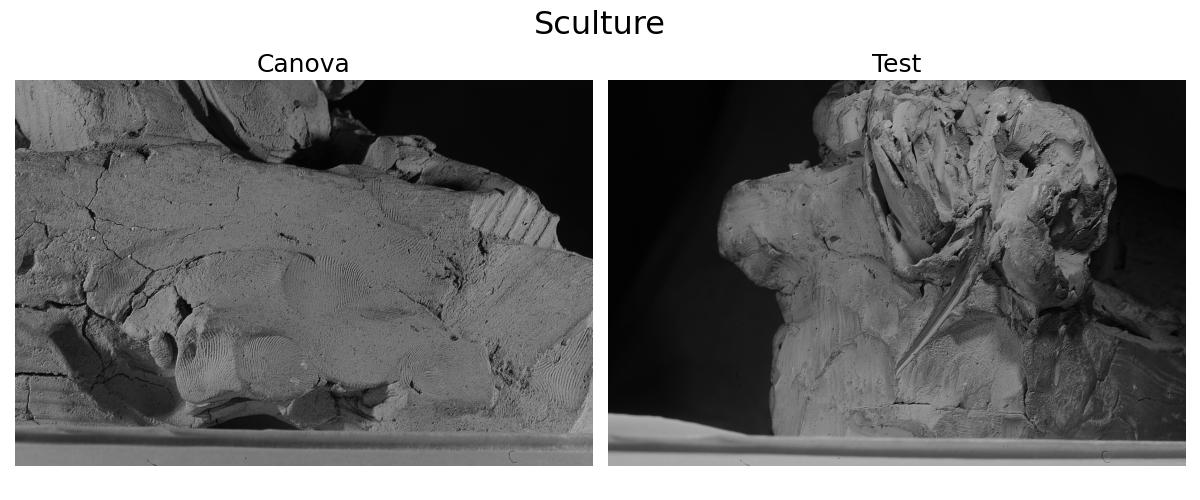
\includegraphics[width=1.0\textwidth]{figures/sculptures.jpg}
    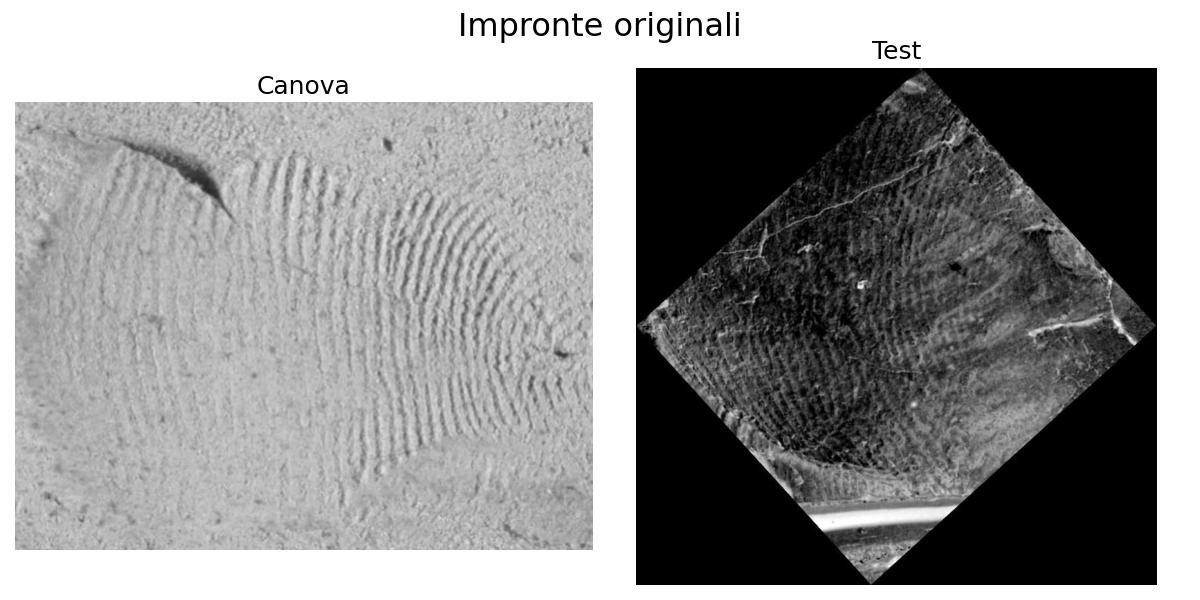
\includegraphics[width=1.0\textwidth]{figures/raw_fingerprints.jpg}
    \caption{Sculture con le impronte di interesse e immagini originali.}
    \label{fig:sculture_rawfp}
\end{figure}

\section*{L'approccio utilizzato}
\noindent
L'approccio storicamente utilizzato per confrontare due impronte era quello di individuare un numero variabile (circa una decina) di \emph{minutiae} in entrambe le impronte. Queste sono punti caratteristici di un'impronta digitale, come biforcazioni o \emph{loop}. Successivamente la corrispondenza veniva verificata da uno o più esperti.

In tempi più recenti, l'articolo del 2012 \emph{Quantifying the weight of evidence from a forensic fingerprint comparison: a new paradigm} di C. Neumann introduce un approccio statistico rigoroso: si costruiscono dei poligoni utilizzando come vertici le \emph{minutiae} individuate, rilevandone misurazioni come angoli, lati e aree; successivamente si utilizza un test basato sul log-rapporto di verosimiglianza per confrontare le misurazioni relative alle due impronte.

Un ulteriore passo avanti è dato dai metodi automatici basati su reti neurali, che si sono dimostrati molto efficaci stabilendosi come stato dell'arte nel settore. Un esempio è VeriFinger, una rete neurale convoluzionale che è disponibile anche come \emph{software} scaricabile con \emph{demo} gratuita.

La situazione in analisi porta con sé delle problematiche legate all'impossibilità di ottenere una scannerizzazione precisa delle impronte di interesse e alla qualità delle immagini stesse. Questo rende impossibile l'utilizzo dei metodi sopra citati. Per superare queste limitazioni si lavora sulle immagini per migliorarne il più possibile la visibilità, successivamente si individuano delle aree con le \emph{minutiae} potenzialmente corrispondenti per entrambe le impronte. Per fare questo, le aree vengono inizialmente individuate sull'immagine con l'impronta di Canova, che risulta più visibile, e successivamente trasferite sulla seconda immagine sfruttando la sovrapposizione fornita dal committente. Il risultato di queste operazioni viene riportato in Figura \ref{fig:boxed_fp}

\begin{figure}[!htb]
    \centering
    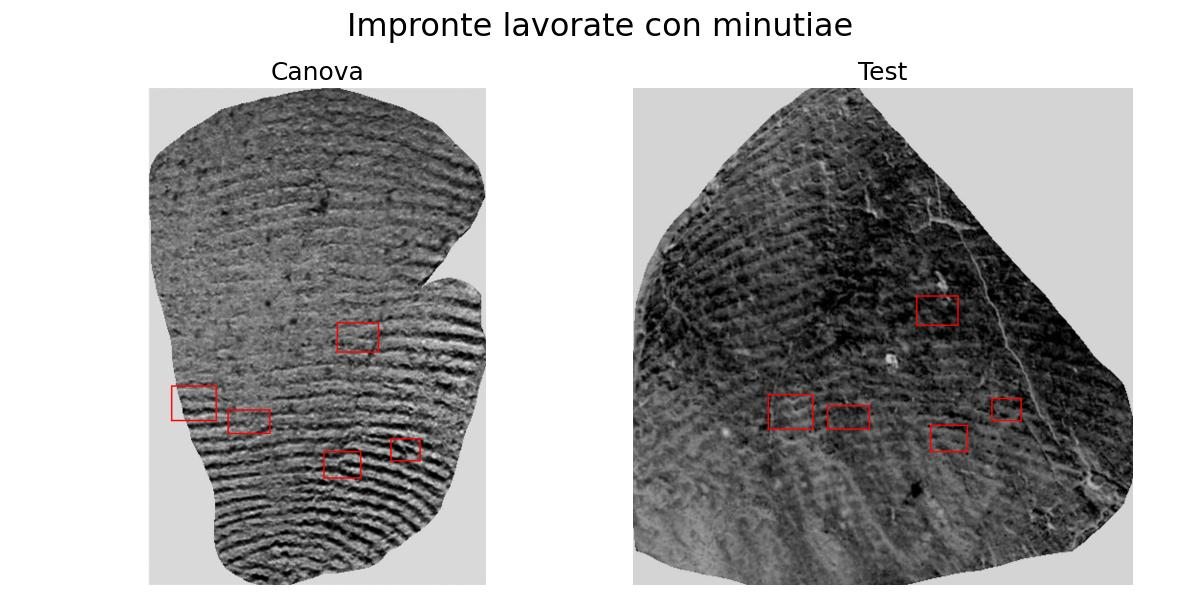
\includegraphics[width=1.0\textwidth]{figures/boxed_fingerprints.jpg}
    \caption{Immagini processate con rettangoli intorno alle \emph{minutiae} di interesse.}
    \label{fig:boxed_fp}
\end{figure}

L'approccio utilizzato per confrontare due rettangoli è il seguente: si trasforma la porzione di immagine contenuta nel rettangolo in un vettore e si effettuano diversi test a due campioni per confrontare il parametro di posizione. L'idea è quella di verificare se l'intensità del colore dei pixel nelle due porzioni è la medesima.

Il sistema di ipotesi è quindi:
\begin{equation*}
    \begin{cases}
        H_0: & \text{le distribuzioni dell'intensità dei pixel hanno la stessa media nelle due immagini}\\
        H_1: & \overline{H_0}\\
    \end{cases}
\end{equation*}

I test utilizzati sono i seguenti:
\begin{itemize}
    \item \emph{t}-test: test per l'uguaglianza del parametro di posizione in due campioni indipendenti, con assunzione di uguale varianza;
    \item Welch's \emph{t}-test: variante robusta del \emph{t}-test che non utilizza l'assunzione di uguale varianza;
    \item Yuen's \emph{t}-test: un'altra variante che utilizza le medie troncate per il confronto (in questo caso si utilizza un troncamento pari a 0.1 per entrambe le code della distribuzione);
    %\item \emph{Mann-Whitney}: test non parametrico basato sui ranghi per verificare se due campioni indipendenti provengono dalla stessa distribuzione;
    \item Kruskal-Wallis: test non parametrico basato sui ranghi per verificare se due campioni indipendenti provengono dalla stessa distribuzione 
\end{itemize}

Il limite di questo metodo è che si perde la nozione sulla località dei pixel. Se per esempio si avesse un'immagine formata da due quadrati adiacenti, uno nero e uno bianco, l'intensità media dei pixel per le due immagini sarebbe la stessa a prescindere dalla posizione dei quadrati. Nonostante questo, l'approccio proposto dovrebbe riuscire a identificare due immagini corrispondenti se una viene ottenuta dall'altra perturbandone i pixel casualmente. Per verificare il funzionamento dell'approccio, si prende il rettangolo 4 dell'impronta di Canova (la numerazione parte dalla \emph{minutia} in alto e va in senso antiorario) e si ottengono diverse perturbazioni dell'immagine aggiungendo ad ogni pixel un valore estratto da una distribuzione normale a media nulla e con deviazione standard crescente. I risultati di questa operazione sono riportati in Figura \ref{fig:proof1}.

\begin{figure}[!htb]
    \centering
    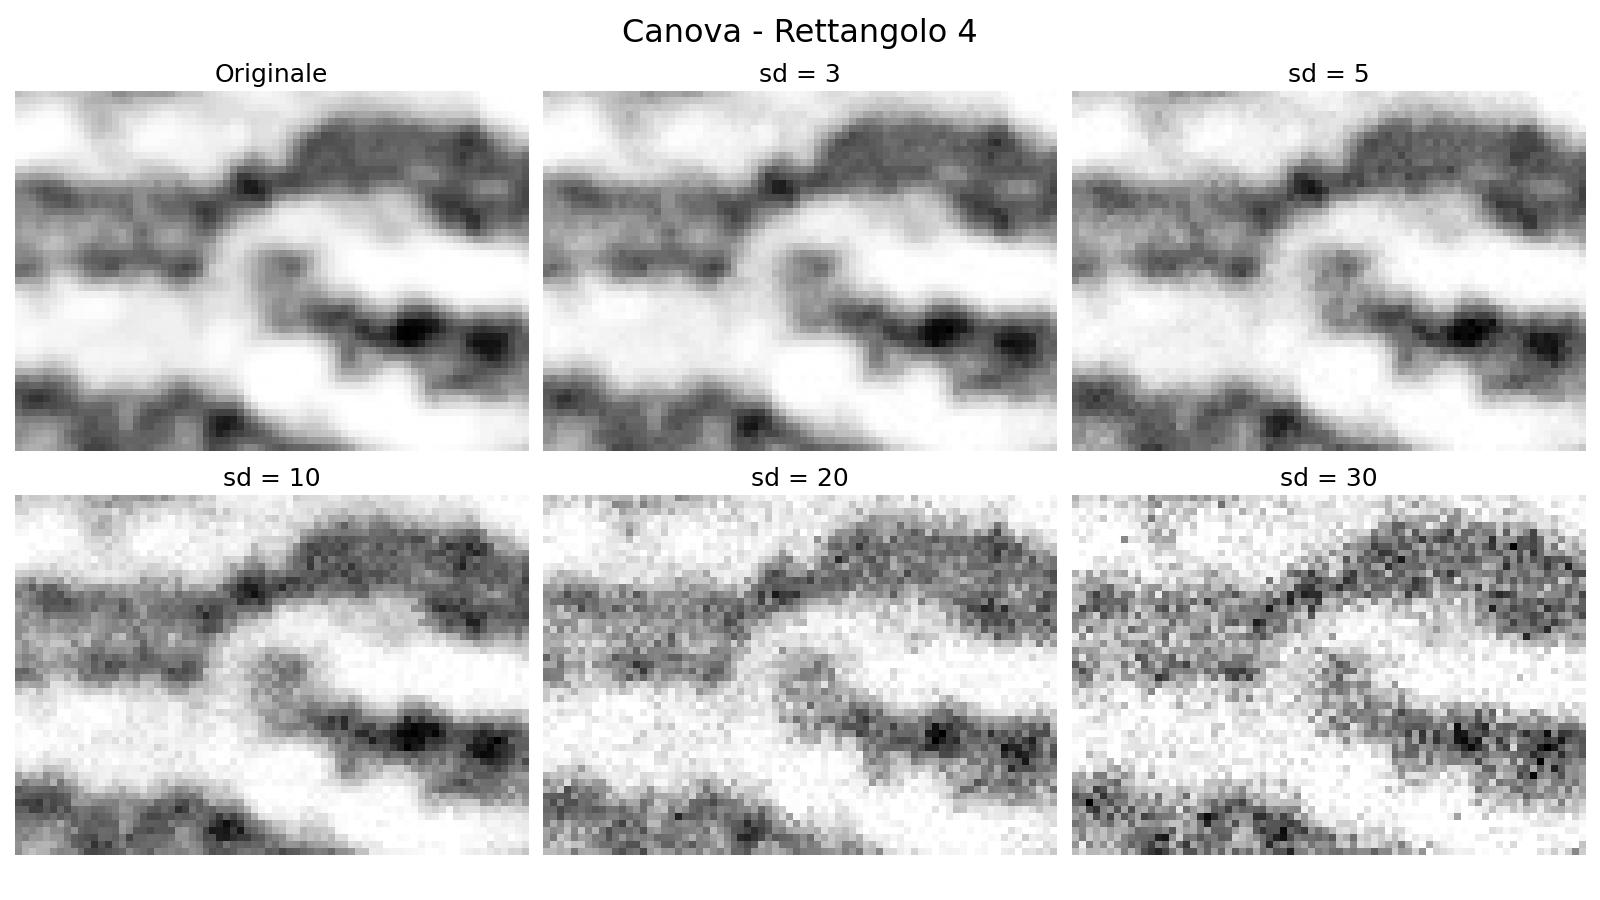
\includegraphics[width=1.0\textwidth]{figures/proof1.jpg}
    \caption{Perturbazioni causali del quarto rettangolo dell'impronta di Canova.}
    \label{fig:proof1}
\end{figure}

In Tabella \ref{tab:proof_of_work} si possono vedere i risultati dei test per i diversi valori di deviazione standard. Per ogni test vengono riportati il valore della statistica di riferimento e tra parentesi il \emph{p-value} associato alla verifica di ipotesi: dai valori elevati di praticamente tutti i \emph{p-value} si vede come i test non rifiutino l'ipotesi di uguaglianza dell'intensità dei pixel con l'immagine originale per tutte le immagini perturbate.

\setlength{\tabcolsep}{8pt}
\begin{table}[!htb]
    \centering
    \begin{tabular}{rrrrr}
        \toprule
        sd & \emph{t}-test & Welch's \emph{t}-test & Yuen's \emph{t}-test &  Kruskal-Wallis \\
        \midrule 
        3 & -0.1012 (0.9194) & -0.1012 (0.9194) & -0.0306 (0.9756) & 0.0467 (0.8289)\\
        5 & -0.0103 (0.9918) & -0.0103 (0.9918) & 0.0603 (0.9519) & 0.0012 (0.9728)\\
        10 & -0.2751 (0.7832) &-0.2751 (0.7832) & -0.0210 (0.9832) & 0.0232 (0.8790)\\
        20 & -1.0006 (0.3171) & -1.0006 (0.3171) & -0.3945 (0.6932) & 0.3850 (0.5350)\\
        30 & -1.8579 (0.0632) & -1.8579 (0.0632) & -0.5678 (0.5702) & 0.5565 (0.4557)\\
        \bottomrule
        \end{tabular}
    \caption{Risultati dei test a due campioni tra la versione originale del rettangolo 4 e le sue perturbazioni.}
    \label{tab:proof_of_work}
\end{table}

In generale si può affermare che, nonostante i limiti derivanti dall'approccio vettoriale, l'approccio utilizzato permette di riconoscere coppie di immagini simili.

\section*{Test sulle impronte}
\noindent
Si procede quindi a ritagliare le due immagini in corrispondenza dei rettangoli individuati e successivamente a prepararle per i test a due campioni. Le coppie di rettangoli vengono visualizzate in Figura \ref{fig:paired_fp}.

\begin{figure}[!htb]
    \centering
    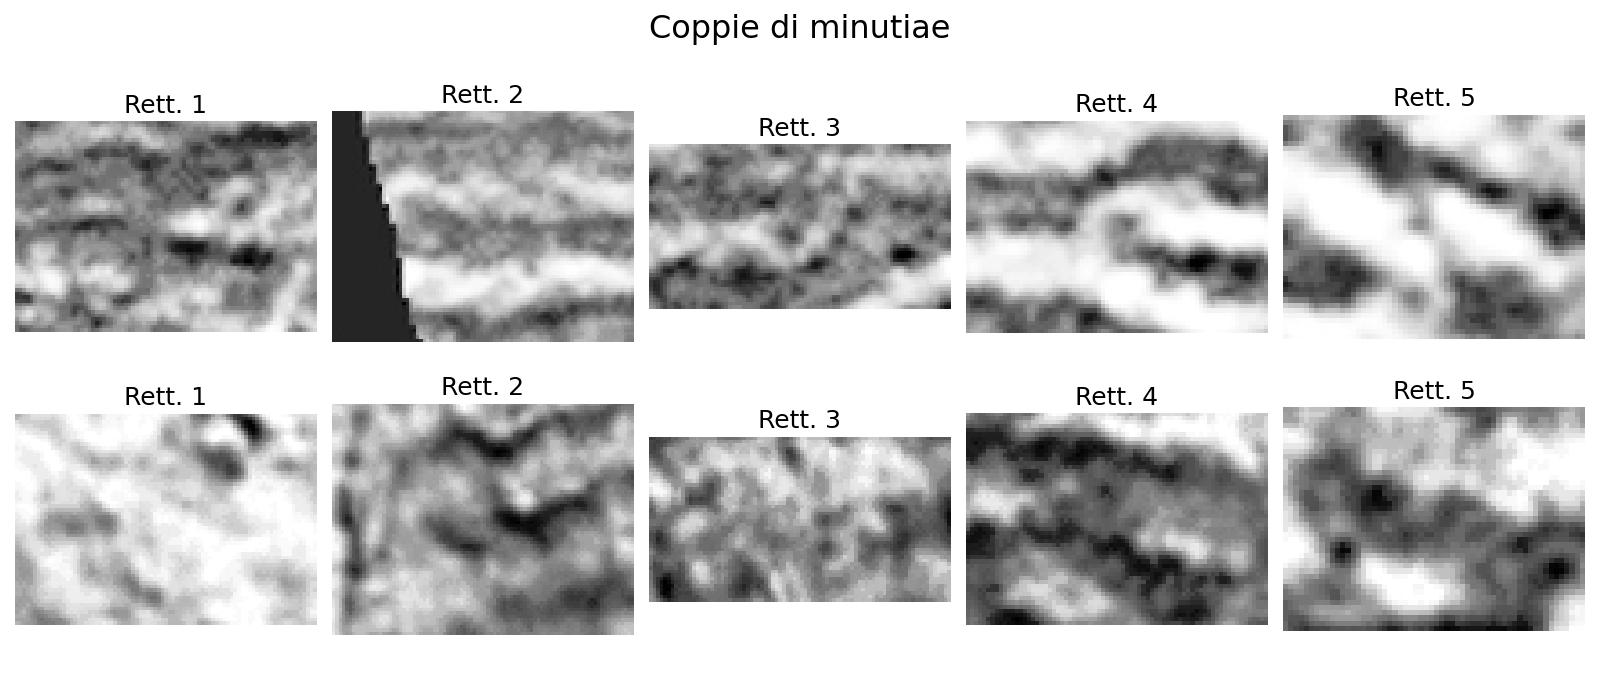
\includegraphics[width=1.0\textwidth]{figures/paired_boxes.jpg}
    \caption{Coppie di rettangoli per le \emph{minutiae} di interesse.}
    \label{fig:paired_fp}
\end{figure}

I risultati dei test vengono riportati in Tabella \ref{tab:two_samples_tests}. Come si vede subito dai valori dei \emph{p-value}, tutti i test rifiutano per tutti i rettangoli considerati l'ipotesi di uguaglianza dei parametri di posizione delle due distribuzioni di riferimento per l'intensità dei pixel. La conseguenza è che l'approccio utilizzato porta a concludere che le due immagini non sono sufficientemente simili e quindi le due impronte non appartengono alla stessa persona.

\setlength{\tabcolsep}{8pt}
\begin{table}[!htb]
    \centering
    \begin{tabular}{rrrrr}
        \toprule
        Rett. & \emph{t}-test & Welch's \emph{t}-test & Yuen's \emph{t}-test &  Kruskal-Wallis \\
        \midrule
        1 & 121.2174 (0.0000) & 121.2174 (0.0000) & 116.8421 (0.0000) & 5924.0893 (0.0000)\\
        2 & 45.4196 (0.0000) & 45.4196 (0.0000) & 45.8374 (0.0000) & 1849.2862 (0.0000)\\
        3 & 77.3186 (0.0000) & 77.3186 (0.0000) & 73.7329 (0.0000) & 3420.5873 (0.0000)\\
        4 & 10.1588 (0.0000) & 10.1588 (0.0000) & 5.7081 (0.0000) & 42.1775 (0.0000)\\
        5 & 19.7645 (0.0000) & 19.7645 (0.0000) & 14.4507 (0.0000) & 205.8371 (0.0000)\\
        \bottomrule
        \end{tabular}
    \caption{Risultati dei test a due campioni sulle coppie di rettangoli.}
    \label{tab:two_samples_tests}
\end{table}

\section*{Commenti finali}
\noindent
Quello che emerge dai test è la presenza di evidenza empirica che porta a rifiutare l'ipotesi iniziale di uguaglianza delle medie dei valori dei pixel, per tutte le \emph{minutiae} considerate. Assumendo come valido l'approccio utilizzato, ne consegue che sulla base dei test non si può affermare che le due impronte provengano dalla stessa persona. In realtà, in virtù delle limitazioni considerate per l'approccio proposto, sarebbe meglio affermare che nella situazione presente a causa della qualità dei dati di partenza non è possibile utilizzare gli strumenti migliori per affrontare il problema, e che l'approccio utilizzato non può essere considerato come completamente affidabile per rispondere al quesito di interesse.

\`E completamente possibile infatti che utilizzando immagini migliori o scansioni, metodi avanzati come VeriFinger evidenzino un effettiva corrispondenza tra le immagini.

\end{document}


